%%%%%%%%%%%%%%%%%%%%%%%%%%%%%%%%%%%%%%%%%
% Beamer Presentation
% LaTeX Template
% Version 1.0 (10/11/12)
%
% This template has been downloaded from:
% http://www.LaTeXTemplates.com
%
% License:
% CC BY-NC-SA 3.0 (http://creativecommons.org/licenses/by-nc-sa/3.0/)
%
%%%%%%%%%%%%%%%%%%%%%%%%%%%%%%%%%%%%%%%%%

%----------------------------------------------------------------------------------------
%	PACKAGES AND THEMES
%----------------------------------------------------------------------------------------

\PassOptionsToPackage{prologue}{xcolor}
%\documentclass[notes,usenames,svgnames,dvipsnames,10pt]{beamer}
\documentclass[usenames,svgnames,dvipsnames,10pt]{beamer}

\usepackage{amsthm,amsmath,amssymb,amscd}

%\usepackage{CustomColors}

\definecolor{indiagreen}{rgb}{0.07,0.53,0.03}
\definecolor{GATechBlue}{rgb}{0.0,0.18823529411764706,0.3411764705882353}%{003057}
\definecolor{GATechGold}{rgb}{0.7019607843137254,0.6392156862745098,0.4117647058823529}%{B3A369​}
\definecolor{GATechBuzzGold}{rgb}{0.9176470588235294,0.6666666666666666,0.0}%{EAAA00}

\mode<presentation> {

% The Beamer class comes with a number of default slide themes
% which change the colors and layouts of slides. Below this is a list
% of all the themes, uncomment each in turn to see what they look like.

%\usetheme{default}
\usetheme{AnnArbor}
%\usetheme{Antibes}
%\usetheme{Bergen}
%\usetheme{Berkeley}
%\usetheme{Berlin}
%\usetheme{Boadilla}
%\usetheme{CambridgeUS}
%\usetheme{Copenhagen}
%\usetheme{Darmstadt}
%\usetheme{Dresden}
%\usetheme{Frankfurt}
%\usetheme{Goettingen}
%\usetheme{Hannover}
%\usetheme{Ilmenau}
%\usetheme{JuanLesPins}
%\usetheme{Luebeck}
%\usetheme{Madrid}
%\usetheme{Malmoe}
%\usetheme{Marburg}
%\usetheme{Montpellier}
%\usetheme{PaloAlto}
%\usetheme{Pittsburgh}
%\usetheme{Rochester}
%\usetheme{Singapore}
%\usetheme{Szeged}
%\usetheme{Warsaw}

% As well as themes, the Beamer class has a number of color themes
% for any slide theme. Uncomment each of these in turn to see how it
% changes the colors of your current slide theme.

%\usecolortheme{albatross}
%\usecolortheme{beaver}
%\usecolortheme{beetle}
%\usecolortheme{crane}
%\usecolortheme{dolphin}
%\usecolortheme{dove}
%\usecolortheme{fly}
%\usecolortheme{lily}
%\usecolortheme{orchid}
%\usecolortheme{rose}
%\usecolortheme{seagull}
%\usecolortheme{seahorse}
%\usecolortheme{whale}
%\usecolortheme{wolverine}

%\setbeamertemplate{footline} % To remove the footer line in all slides uncomment this line
%\setbeamertemplate{footline}[page number] % To replace the footer line in all slides with a simple slide count uncomment this line

%\setbeamertemplate{navigation symbols}{} % To remove the navigation symbols from the bottom of all slides uncomment this line

\setbeamercolor*{structure}{bg=GATechBlue,fg=GATechGold}

\setbeamercolor*{palette primary}{use=structure,fg=white,bg=structure.fg}
\setbeamercolor*{palette secondary}{use=structure,fg=white,bg=GATechGold!85!black}
\setbeamercolor*{palette tertiary}{use=structure,fg=white,bg=GATechGold!70!black}
\setbeamercolor*{palette quaternary}{fg=white,bg=GATechGold!65!white}

\setbeamercolor{frametitle}{bg=GATechBlue,fg=GATechBuzzGold}
\setbeamercolor*{titlelike}{bg=GATechBlue,fg=GATechBuzzGold}

\defbeamertemplate{itemize item}{bulletpoint}{\usebeamerfont*{itemize item enumitem}\raise1.05pt\hbox{\color{GATechGold!70!black}{$\blacktriangleright$}}}
\setbeamertemplate{items}[bulletpoint]

\setbeamercolor{section in toc}{fg=black}
\setbeamercolor{subsection in toc}{fg=black}

\setbeamercolor{bibliography item}{parent=palette primary}
\setbeamercolor{bibliography entry author}{fg=GATechBlue}
\setbeamercolor{bibliography entry title}{fg=GATechBlue}
\setbeamercolor{bibliography entry note}{fg=GATechBlue}

}

\usepackage{graphicx} % Allows including images
\usepackage{booktabs} % Allows the use of \toprule, \midrule and \bottomrule in tables
\usepackage{fancyvrb}
\usepackage{inconsolata}

\newcommand{\Iverson}[1]{\ensuremath{\left[#1\right]_{\delta}}} 

\DeclareMathOperator{\DGF}{DGF} 
\DeclareMathOperator{\ds}{ds} 
\DeclareMathOperator{\Id}{Id}
\DeclareMathOperator{\sq}{sq}

\newcommand{\ceiling}[1]{\ensuremath{\left\lceil #1 \right\rceil}} 
\newcommand{\ImportantMarker}{%\textcolor{GATechGold}{$\mathbf{\Leftarrow}$}\ 
                              \textcolor{GATechGold}{\textbf{[!! \underline{IMPORTANT} !!]}}}

\newcommand{\Floor}[2]{\ensuremath{\left\lfloor \frac{#1}{#2} \right\rfloor}}
\newcommand{\Ceiling}[2]{\ensuremath{\left\lceil \frac{#1}{#2} \right\rceil}}                              

\newcommand{\gkpSI}[2]{\ensuremath{\genfrac{\lbrack}{\rbrack}{0pt}{}{#1}{#2}}} 
\newcommand{\gkpSII}[2]{\ensuremath{\genfrac{\lbrace}{\rbrace}{0pt}{}{#1}{#2}}}

\newcommand{\TitleBoxed}[1]{
     \begin{beamercolorbox}[sep=8pt,center,shadow=true,rounded=true]{title}
          \usebeamerfont{title}#1\vskip 0.6cm\par%
     \end{beamercolorbox}
}

\usepackage{listings}
\definecolor{codeEnvBGColor}{rgb}{0.0,0.82,0.67}
\lstnewenvironment{code}{%
  \lstset{backgroundcolor=\color{codeEnvBGColor},
  frame=single,
  framerule=0pt,
  basicstyle=\ttfamily\scriptsize,
  breaklines=true,
  columns=fullflexible}}{}
\definecolor{pythonCodeEnvBGColor}{gray}{0.85}
\lstnewenvironment{pythoncode}{%
  \lstset{backgroundcolor=\color{pythonCodeEnvBGColor},
  frame=single,
  framerule=0pt,
  numbers=left,
  xleftmargin=1.9em,
  framexleftmargin=1.9em,
  stepnumber=1,
  basicstyle=\ttfamily\small,
  breaklines=true,
  language=Python}}{}
\lstnewenvironment{pythoncodesmall}{%
  \lstset{backgroundcolor=\color{pythonCodeEnvBGColor},
  frame=single,
  framerule=0pt,
  numbers=left,
  xleftmargin=3.5em,
  framexleftmargin=3.5em,
  stepnumber=1,
  basicstyle=\ttfamily\tiny,
  breaklines=true,
  language=Python}}{}

%\setbeamertemplate{note page}[plain]
\setbeamerfont{note page}{family*=pplx,size=\footnotesize} % Palatino for notes

%----------------------------------------------------------------------------------------
%	TITLE PAGE
%----------------------------------------------------------------------------------------

\title[Math 6307 Course Project]{
     Math 6307 Course Project: \\ Modern methods of exploration of numerical ODE solutions using Python3 
} 

\author{Maxie Dion Schmidt} % Your name
\institute[GA Tech] 
{
Georgia Institute of Technology \\ 
School of Mathematics \\ % Your institution for the title page
\medskip
\textit{maxieds@gmail.com} \\ 
\textit{mschmidt34@gatech.edu} \\ 
\medskip 
\url{http://people.math.gatech.edu/~mschmidt34/} \\ 
\url{https://github.com/maxieds/GATechMath6307ODEsCourseProject}
}
\date[November 2, 2021]{November 2, 2021 \\ {\small{\it (Last compiled with \LaTeX2e on \today)}}} % Date, can be changed to a custom date

\begin{document}

\begin{frame}
\titlepage % Print the title page as the first slide
%\note[item]{No notes for this page}
\end{frame} 

%----------------------------------------------------------------------------------------
%	PRESENTATION SLIDES
%----------------------------------------------------------------------------------------

%------------------------------------------------

\section{Overview and goals of the presentation} 

\begin{frame}
     \frametitle{Goals of the presentation}

\begin{itemize} 

     \item Explore options of modern packages for Python3 that facilitate exploring ODE (systems of ODEs) solutions numerically 
     \item Give a few examples of generic, \emph{\textbf{re-usable}} numerical methods for a toy 1D ODE problem
     \item Define and motivate the study of \emph{chaotic attractors} (corresponding to parameterized multidimensional systems of ODEs -- 
           typically 3D and 4D in a time variable, or 2D projections of such systems) 
     \item Show some particular experiment types for the \emph{R\"ossler attractor} that can be extended to other applications and use cases
     \item All source code, presentation materials and package install notes 
           for this project are freely available under the GPL-V3 at \\ 
           {\small{\url{https://github.com/maxieds/GATechMath6307ODEsCourseProject}}}

\end{itemize} 

\end{frame}

\section{Examples of solving ODEs in Python3}

\begin{frame}
\frametitle{Basic examples} 

\TitleBoxed{
     \Large{\centerline{Basic examples of solving ODEs in Python3}}
}

\end{frame}

\subsection{Setup: Model problem}

\begin{frame}
\frametitle{Setup: Defining a common model problem}

\begin{itemize} 

\item Typically we look at an IVP of the following form: \\ 
      $y^{\prime} = f(t, y), y(t_0) = y_0$
\item For the purposes of exploring our options in Python3, we will take a 
      special case of this problem type
\item The special case is defined for some parameter $k$ as: \\ 
     $y^{\prime} = (t-y^k)(3-ty-2y^2)$ subject to $y(0) = 1$ 
\item That is: $f(t, y) := (t-y^k)(3-ty-2y^2)$ with $(t_0, y_0) := (0, 1)$
\item The analysis of this ``toy'' model problem facilitates comparing the functionality and 
      ease of use for numerically approximating its solutions (for various fixed $k$) 
      of common libraries and algorithms in Python3

\end{itemize} 

\note[item]{No notes for this page}

\end{frame}

\subsection{Explicit forward Euler method}

\begin{frame}
\frametitle{Explicit forward Euler method}

\begin{itemize} 

\item Given an IVP: $y^{\prime} = f(t, y), y(t_0) = y_0$ 
\item The forward Euler method is an explicit method for iteratively 
      generating numerical solutions to this ODE provided that we can 
      evaluate $f$ clearly 
\item Convergence to solution and other numerical analysis of the algorithm 
      (e.g., LTE and GTE truncation errors at each step) and 
      corresponding accuracy given fixed $h$ is standard reading 
\item $y_{n+1} = y_n + f(t_n, y_n) \left(t_{n+1} - t_n\right) = y_n + h \cdot f(t_n, y_n)$ 

\end{itemize} 

\end{frame}

\begin{frame}
\frametitle{Explicit forward Euler method -- Motivation}

\begin{itemize} 

\item \textbf{\underline{Key derivation}:} $y^{\prime}(t_0) \approx \frac{y(t_0+h)-y(t_0)}{h}$ ($\ast$), where 
      $y^{\prime} = f(t, y)$ $\implies$ $y(t_0+h)-y(t_0) \approx \int_{t_0}^{t_0+h} f(t, y(t)) dt$ 
\item Now we approximate the the RHS integral using a left-hand-endpoint Riemann sum ($n=1$ rectangle) to 
      obtain that $\int_{t_0}^{t_0+h} f(t, y(t)) dt \approx h \cdot f(t_0, y(t_0))$
\item Forward Euler is the simplest method using this line of reasoning 
\item Modifications can be given, including 
      taking $y^{\prime}\left(t + \frac{h}{2}\right) \approx \frac{y(t+h)-y(t)}{h}$ in place of ($\ast$) above, 
      leading to the \emph{midpoint method} 
\item Implicit backwards Euler forms another variant 

\end{itemize} 

\end{frame}

\begin{frame}[fragile]
\frametitle{Explicit foward Euler method (source code flavor)}

\begin{center}
\begin{pythoncode}
def ExplicitForwardEuler(ftyFunc, icPoint, solInterval, h):
    f = ftyFunc
    (t0, y0) = icPoint
    (solA, solB) = solInterval
    numGridPoints = math.floor(float((solB - solA) / h))
    tPoints = np.linspace(solA, solB, numGridPoints + 1)
    yPoints = [ y0 ]
    curYn = y0
    for n in range(0, numGridPoints):
        tn = tPoints[n]
        nextYn = curYn + f(tn, curYn) * h
        yPoints += [ nextYn ]
        curYn = nextYn
    # ... Matplotlib plotting code for the solution ... 
\end{pythoncode}
\end{center}

\end{frame}

\begin{frame}[fragile]
\frametitle{Explicit foward Euler method (results)}

\begin{center}
\begin{code}
(ipython) cd Examples/BasicNumericalODESolutionMethods
(ipython) run "ExplicitForwardEulerMethod.py"
\end{code}
\vskip -0.205cm
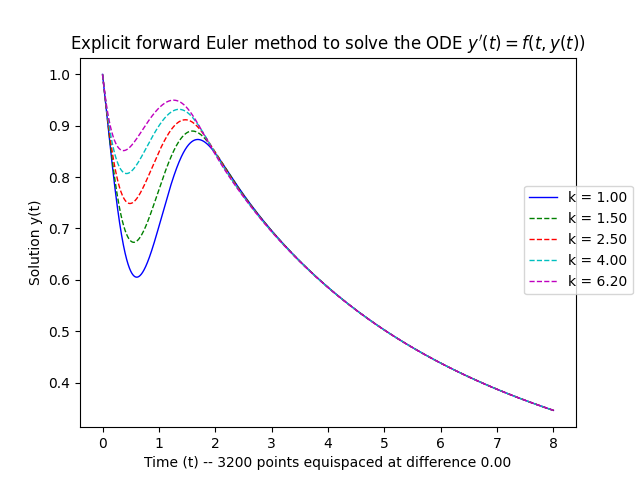
\includegraphics[height=0.76\textheight]{../Images/ExplicitForwardEuler-PlotOutput-v1.png}
\end{center}

\end{frame}

\subsection{Runga-Kutta (RK4) method}

\begin{frame}
\frametitle{Runga-Kutta (RK4) method}

\begin{itemize} 

\item Given an IVP: $y^{\prime} = f(t, y), y(t_0) = y_0$ 
\item $t_n = t_0 +h \cdot n$ (fixed / uniform step size)
\item $k_1 = f(t_n, y_n)$, $k_2 = f\left(t_n + \frac{h}{2}, y_n + \frac{k_1h}{2}\right)$, 
      $k_3 = f\left(t_n + \frac{h}{2}, y_n + \frac{k_2h}{2}\right)$, $k_4 = f\left(t_n + h, y_n + k_3h\right) $ 
\item $y_{n+1} = y_n + \frac{h}{6}\left(k_1 + 2k_2 + 2k_3 + k_4\right)$ (recursion to evaluate) 
\item Taking the weighted average at four slopes leads to more weight given to slopes closer to the midpoint 
      of each subinterval 
\item $\operatorname{LTE} = O(h^5)$ and $\operatorname{AccumulatedTruncationError} = O(h^4)$ 
\item If $f$ does not depend on $y$, the RK4 is the same as \emph{Simpson's rule} 

\end{itemize} 

\end{frame}

\subsection{Runga-Kutta (RK4) method}

\begin{frame}
\frametitle{More general explicit Runga-Kutta methods}

\begin{itemize} 

\item The family of \emph{explicit RK methods} ($s$-stage) is paramterized by: \\ 
      $y_{n+1} = y_n + \sum\limits_{i=1}^{s} hb_ik_i$ where \\ 
      $k_1 = f(t_n, y_n)$ \\ 
      $k_2 = f(t_n + c_2h, y_n +h \cdot (a_{21}k_1))$ \\ 
      $k_3 = f(t_n + c_3h, y_n + h \cdot (a_{31}k_1 + a_{32}k_2))$ \\ 
      $\phantom{k_4}\cdots$ \\ 
      $k_s = f(t_n + c_sh, h \cdot(a_{s1}k_1 + a_{s2}k_2 + \cdots + a_{s,s-1}k_{s-1}))$. 
\item That is, the explicit RK method is completely determined by the parameters 
      $(a_{ij})_{1 \leq j < i \leq s}$, $(b_i)_{1 \leq i \leq s}$ and $(c_j)_{2 \leq j \leq s}$
\item We require \emph{consistency} insomuch as $\sum\limits_{i=1}^s b_i = 1$ 
\item A popular convention is to require that $\sum\limits_{j=1}^{i-1} a_{ij} = c_i$ for $i \in \{2,3,\ldots,s\}$ 
%\item \textbf{Variants:}  
%      There also exist second-order RK methods with two stages, adaptive RK methods, implicit RK methods 
%      (each has its own set of properties and advantages/disadvantages per use case, e.g., stability requirements)

\end{itemize} 

\end{frame}
\begin{frame}[fragile]
\frametitle{Runga-Kutta (RK4) method (source code flavor)}

\begin{center}
\begin{pythoncode}
def RungeKuttaRK4(ftyFunc, icPoint, solInterval, h):
    f = ftyFunc
    (t0, y0) = icPoint
    (solA, solB) = solInterval
    numGridPoints = math.floor(float((solB - solA) / h))
    tPoints = np.linspace(solA, solB, numGridPoints + 1)
    yPoints = [ y0 ]
    curYn = y0
    for n in range(0, numGridPoints):
        tn = tPoints[n]
        k1 = f(tn, curYn)
        k2 = f(tn + h / 2.0, curYn + k1 * h / 2.0)
        k3 = f(tn + h / 2.0, curYn + k2 * h / 2.0)
        k4 = f(tn + h, curYn + k3 * h)
        nextYn = curYn + h / 6.0 * (k1 + 2 * k2 + 2 * k3 + k4)
        yPoints += [ nextYn ]
        curYn = nextYn
\end{pythoncode}
\end{center}

\end{frame}

\begin{frame}[fragile]
\frametitle{Runga-Kutta (RK4) method (results)}

\begin{center}
\begin{code}
(ipython) cd Examples/BasicNumericalODESolutionMethods
(ipython) run "ImplicitRungeKuttaMethod.py"
\end{code}
\vskip -0.205cm
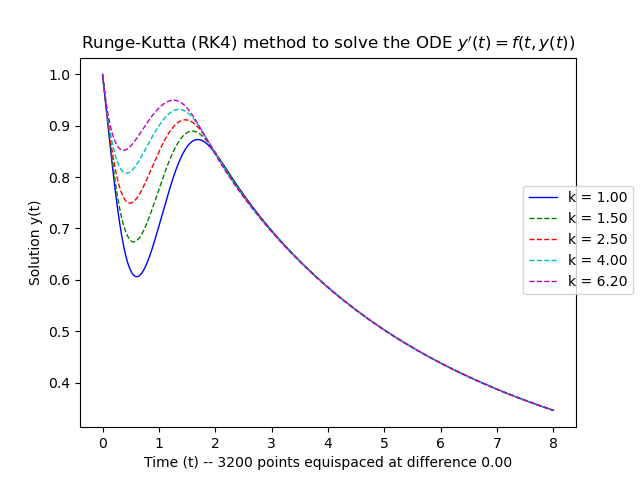
\includegraphics[height=0.76\textheight]{../Images/ImplicitRungeKuttaRK4RecursionFormula-PlotOutputs-v2.png}
\end{center}

\end{frame}

\subsection{Linear multistep solver method (general model and ABF-3)}

\begin{frame}
\frametitle{Overview of general multistep methods}

\begin{itemize} 

\item General multistep method with $s$ steps: 
      $$y_{n+s} + \sum\limits_{j=0}^{s-1} a_j y_{n+j} = \sum\limits_{m=0}^s hb_m f(t_{n+m}, y_{n+m})$$
\item Polynomial interpolation: 
      $$p(t_{n+i}) := f(t_{n+i}, y_{n+i}), \text{ for } i \in \{0,1,\ldots,s-1\}$$
\item Lagrange's exact polynomial interpolation formula under this requirement: 
      $$p(t) = \sum\limits_{0 \leq j < s} \frac{(-1)^{s-j-1} f(t_{n+j}, y_{n+j})}{j! (s-j-1)! h^{s-1}} \times 
       \prod\limits_{\substack{0 \leq i < s \\ i \neq j}} (t-t_{n+i})$$ 
\item Approximations to initial conditions and foundation for building the numerical solutions: 
      $$y_{n} = y_{n-1} + \int\limits_{t_{n-1}}^{t_{n}} p(t) dt, \text{ for } n \in \{1, 2, \ldots, s-1\}$$ 

\end{itemize} 

\end{frame}

\begin{frame}
\frametitle{Step solver method -- Adams-Bashforth (ABF-$s$)}

\begin{itemize} 

\item The multistep ABF-$s$ ($s$-step) case: $a_{s-1}=-1$; $a_{s-2}=\cdots=a_0=0$
\item The multistep ABF-$s$ ($s$-step) case: 
      Substitute $f(t_{n+j}, y_{n+j}) \mapsto p(t_{n+j})$ in the Lagrange interpolation formula from above 
\item The ABF-$s$ method coefficient multipliers yield: 
      $$b_{s-j-1} = \frac{(-1)^j}{j!(s-j-1)!} \times \int\limits_0^1 \prod\limits_{\substack{0 \leq i < s \\ i \neq j}} (u+i) du, 
       \text{ for } j \in \{0,1,\ldots,s-1\}$$ 
\item Recursion in the ABF-3 method: 
      $$y_{n+3} = y_{n+2} + h\left(\frac{23}{12}f(t_{n+2},y_{n+2}) - \frac{4}{3} f(t_{n+1},y_{n+1}) + \frac{5}{12} f(t_n, y_n)\right)$$ 
\item \textbf{Note:} Single step ABF-1 is the forward Euler method 

\end{itemize} 

\end{frame}

\begin{frame}[fragile]
\frametitle{Step solver method -- ABF3 (source code flavor)}

\begin{center}
\begin{pythoncodesmall}
def LagrangePolynomialInterpolation(ftyFunc, numStepsS, prevYPoints, t0, h, n):
    f             = ftyFunc
    s             = numStepsS 
    yPoints       = prevYPoints
    tDiffProdFunc = lambda t, j: reduce(operator.mul, [ t - (t0 + h * (n + i)) if i != j else 1 for i in range(0, s) ])
    ptFunc        = lambda t: sum([ (-1)**(s-j-1) * f(t0 + h * (n + j), yPoints[n+j]) / factorial(j) / \
                                    factorial(s-j-1) / (h**(s-1)) * tDiffProdFunc(t, j) \
                                    for j in range(0, n + len(yPoints)) ])
    nextYPoints   = []
    lastYPoint    = prevYPoints[-1]
    for sidx in range(0, s):
        tnpim1 = t0 + h * (n + sidx - 1)
        tnpi = t0 + h * (n + sidx)
        ynpi = lastYPoint + sympy.integrate(ptFunc(tvar), (tvar, tnpim1, tnpi))
        yPoints += [ ynpi ]
        nextYPoints += [ ynpi ]
        lastYPoint = ynpi
    return nextYPoints
def AdamsBashforthABF3(ftyFunc, icPoint, solInterval, h):
    f             = ftyFunc
    s             = 3
    (t0, y0)      = icPoint
    (solA, solB)  = solInterval
    numGridPoints = math.floor(float((solB - solA) / h))
    tPoints       = np.linspace(solA, solB, numGridPoints + 1)
    yPoints       = [ y0 ] + LagrangePolynomialInterpolation(f, s-1, [ y0 ], t0, h, n=0)
    curYn         = y0
    for n in range(0, numGridPoints + 1 - s):
        tn2, tn1, tn = tPoints[n+2], tPoints[n+1], tPoints[n]
        yn2, yn1, yn = yPoints[n+2], yPoints[n+1], yPoints[n]
        fn2, fn1, fn = f(tn2, yn2), f(tn1, yn1), f(tn, yn)
        nextYn = yn2 + h * (23.0 / 12.0 * fn2 - 4.0 / 3.0 * fn1 + 5.0 / 12.0 * fn)
        yPoints += [ nextYn ]
\end{pythoncodesmall}
\end{center}

\end{frame}

\begin{frame}[fragile]
\frametitle{Step solver method -- ABF3 (results)}

\begin{center}
\begin{code}
(ipython) cd Examples/BasicNumericalODESolutionMethods
(ipython) run "ImplicitStepSolverMethod.py"
\end{code}
\vskip -0.205cm
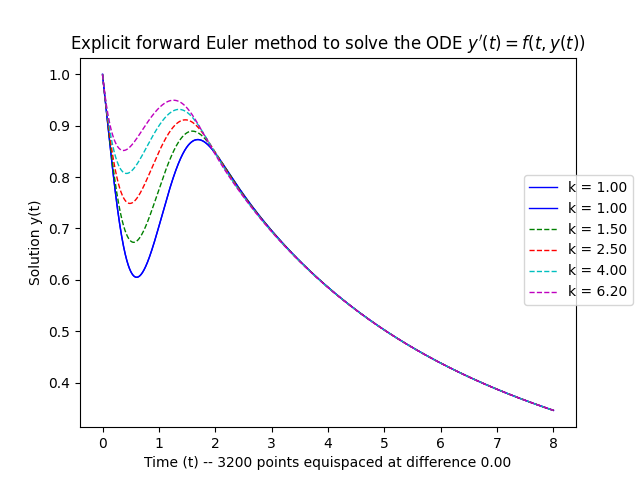
\includegraphics[height=0.76\textheight]{../Images/ABF3MultistepMethodResults-v2.png}
\end{center}

\end{frame}

\subsection{GEKKO library / Python package} 

\begin{frame}[fragile]
\frametitle{GEKKO library (source code flavor)}

\begin{center}
\begin{pythoncodesmall}
gk = GEKKO(remote=False)
def yPowerODEFunc(kpow):
    return lambda t, y: (t - y**kpow) * (3 - y * t - 2 * (y**2))
if __name__ == "__main__":
    kPowParams    = [ 1.0, 1.5, 2.5 ]
    drawStyles    = [ GetDistinctDrawStyle(n) for n in range(0, len(kPowParams)) ]
    gridSpacingH  = 0.001
    solInterval   = (0, 6.0)
    (solA, solB)  = solInterval
    icPoint       = (0, 1)
    (t0, y0)      = icPoint
    numGridPoints = math.floor(float((solB - solA) / gridSpacingH))
    gk.options.IMODE = 4
    gk.options.TIME_SHIFT = 0
    gk.options.SOLVER = 1
    axFig = plt.figure(1)
    for (kidx, kpow) in enumerate(kPowParams):
        k             = gk.Param()
        y             = gk.Var(value=y0)
        gk.time       = np.linspace(solA, solB, numGridPoints + 1)
        t             = gk.Param(value=gk.time)
        k.value       = kpow
        ftyFunc       = yPowerODEFunc(k)(t, y)
        gk.Equation(y.dt() == ftyFunc)
        gk.options.MAX_ITER = 250 * math.floor(kpow) 
        gk.solve(disp=VERBOSE)
        pltDrawStyle = drawStyles[kidx]
        pltLegendLabel = "k = %1.2f" % kpow
        plt.plot(gk.time, y, pltDrawStyle, label=pltLegendLabel, linewidth=1)
    plt.xlabel("Time (t) -- %d points equispaced at difference %1.2f" % (numGridPoints, gridSpacingH))
    plt.ylabel('Solution y(t)')
    plt.title(r'Explicit forward Euler method to solve the ODE $y^{\prime}(t) = f(t, y(t))$')
    axFig.legend(loc='center right')
    plt.show()
\end{pythoncodesmall}
\end{center}

\end{frame}

\begin{frame}[fragile]
\frametitle{GEKKO library (results)}

\begin{center}
\begin{code}
(ipython) cd Examples/BasicNumericalODESolutionMethods
(ipython) run "PythonGEKKOSolver.py"
\end{code}
\vskip -0.205cm
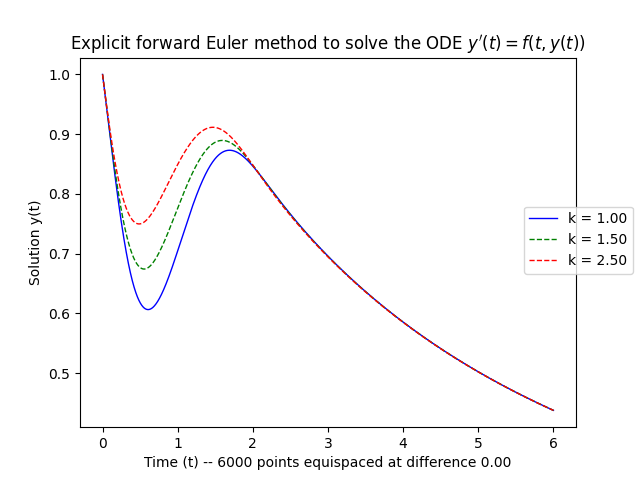
\includegraphics[height=0.76\textheight]{../Images/GEKKOPlotOutputs-v1.png}
\end{center}

\end{frame}


\subsection{Vector field plots from the midterm} 

\begin{frame}
\frametitle{Generating vector field plots for 2D systems}

\begin{itemize} 

\item \emph{\textbf{Problem 4 from the midterm:}} 
      Consider the non-linear ODE $\dot{x} = F(x)$ on $\mathbb{R}^2$ defined such that 
      $F(x, y) = \left(x(1-x^2-y^2)-y, y(1-x^2-y^2)+x\right)^T$
\item The function $F(x, y)$ defines a vector field in 2D 
\item Solutions $(x(t), y(t))$ are witnessed along a hyperbola as can be seen by evaluating the 
      system of equations in polar coordinate 
\item We can get to initial grips with the solutions to this problem and 
      visualize the vector field at hand using standard plotting functions in 
      \texttt{matplotlib.pyplot} (imported as \texttt{plt}) 

\end{itemize} 

\end{frame}

\begin{frame}[fragile]
\frametitle{Generating vector field plots (source code flavor)}

\begin{center}
\begin{pythoncodesmall}
from scipy.integrate import odeint

def PlotVectorField(FxyFunc, xRange, yRange):
    Fxy = lambda x, y: np.array(list(FxyFunc(x, y)))
    xGridPoints, yGridPoints = np.meshgrid(xRange, yRange)
    xv, yv = sympy.var('x y')
    (uQuiver, vQuiver) = Fxy(xGridPoints, yGridPoints)
    xmin, xmax = min(xGridPoints.flatten()), max(xGridPoints.flatten())
    ymin, ymax = min(yGridPoints.flatten()), max(yGridPoints.flatten())
    plt.xlim(xmin, xmax)
    plt.ylim(ymin, ymax)
    plt.quiver(xGridPoints, yGridPoints, uQuiver, vQuiver)
    plt.streamplot(xGridPoints, yGridPoints, uQuiver, vQuiver)

def SolveODE2DSystemWithVectorField(FxyFunc, icPoint, solInterval, h):
    Fxy = lambda s, time: FxyFunc(s[0], s[1])
    (t0, (x0, y0)) = icPoint
    (solA, solB) = solInterval
    numGridPoints = math.floor(float((solB - solA) / h))
    timeSpecT = np.linspace(solA, solB, numGridPoints + 1)
    odeIntSol = odeint(Fxy, [ x0, y0 ], timeSpecT)
    xtSolPoints = odeIntSol[:, 0] 
    ytSolPoints = odeIntSol[:, 1]
    axFig = plt.figure(1) 
    plt.xlabel(r'Time (t)')
    plt.plot(timeSpecT, xtSolPoints, GetDistinctDrawStyle(2), label=r'$x(t)$')
    plt.plot(timeSpecT, ytSolPoints, GetDistinctDrawStyle(6), label=r'$y(t)$')
\end{pythoncodesmall}
\end{center}

\end{frame}

\begin{frame}[fragile]
\frametitle{Results}

\begin{center}
\begin{code}
(ipython) cd Examples/BasicNumericalODESolutionMethods
(ipython) run "ExploringVectorFieldsAndODESystems.py"
\end{code}
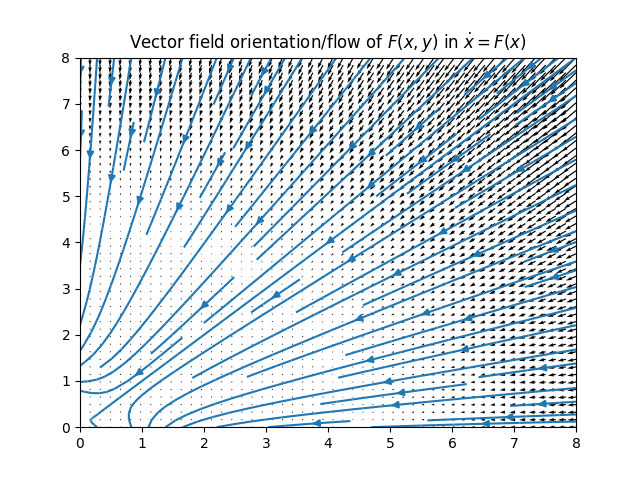
\includegraphics[width=0.49\textwidth]{../Images/Exploring2DSolutionsExample-VectorFieldPlots-v1.png}
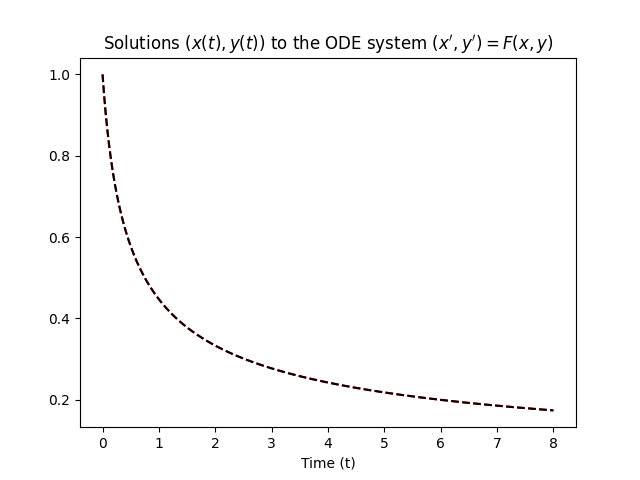
\includegraphics[width=0.49\textwidth]{../Images/Exploring2DSystemSolutions-xtytSolutionPlots-v2.png}
\end{center}

{\small 
The \texttt{plt.quiver} function shows the magnitude of the vectors (as black arrows, above left) 
where the \texttt{plt.streamplot} shows the orientation/directions of the flow of the field 
without indicating magnitudes along the curves (in blue, above left) 
}

\end{frame}


\section{Chaotic Attractors} 

\begin{frame}
\frametitle{Key applications for numerical exploration} 

\TitleBoxed{
     \huge{\centerline{Chaotic attractors}}
}

\end{frame}

\begin{frame}
\frametitle{Definitions and motivation}

\begin{itemize} 

\item A very precise definition of \emph{chaotic attractor} is developed using criteria based on 
      topological constructions in the references (see \cite{CATTR-SURVEY,CHAOS-BOOK})
\item We will stick to a high-level qualitative description motivating study of the behavior of systems of this type 
\item When considering dynamical systems, an \emph{attractor} is a set of states (orbits) towards which a system (of ODE solutions) 
      tends to evolve
\item System values within some small range of the \emph{attractor} set stay close even if perturbed slightly 
      (e.g., by slightly shifting an ODE initial condition) 
\item A \emph{chaotic attractor} is correspondingly an attractor admitting system that exhibit apparently randomized behavior and 
      disorderly irregularities in form 
\item Systems that form a \emph{chaotic attractor} type are highly sensitive to initial conditions 

\end{itemize} 

\end{frame}

\begin{frame}
\frametitle{Famous examples of chaotic attractors}

\begin{itemize} 

\item We will focus on numerical exploration of the \emph{R\"ossler attractor} system 
\item Other famous examples that extend applications of these numerical ideas in Python 3 
      include the following chaotic attractor system variants: \\ 
      The \emph{Robin attractor}, the \emph{Lorenz--63 model} (3D solutions), and 
      the \emph{Lorenz--96 model}
\item There is much on these special cases in the literature (we do not have enough time to cover them all here) 

\end{itemize} 

\end{frame}

\section{The R\"ossler Attractor} 


\begin{frame}
\frametitle{Our prototype attractor problem for numerical investgation} 

\TitleBoxed{
     \huge{\centerline{Key application: The R\"ossler attractor}}
}

\end{frame}

\subsection{Definitions} 

\begin{frame}
\frametitle{Definition of the R\"ossler attractor problem}

\begin{itemize} 

\item Non-linear 3D systems of ODEs determined by parameters $(a, b, c) \in \mathbb{R}^3$ 
\item Precise system: $(x^{\prime}, y^{\prime}, z^{\prime}) = (-y-z, x+ay, b + z(x-c))$ 
\item R\"ossler famously studied the ``classic'' case with $(a, b, c) := (0.2, 0.2, 5.7)$ 
      (important characteristic properties of other parameter special cases are known) 
\item Often times to simplify considerations, we consider a projection of the system corresponding to 
      setting one of the $XYZ$-components to zero, e.g., the projection in the $XY$-plane seen by setting 
      $z := 0$ 

\end{itemize} 

\end{frame}

\subsection{Numerical exploration of solutions} 

\begin{frame}[fragile]
\frametitle{Preliminary numerical exploration of solutions}

\begin{itemize} 

\item We can use the \texttt{scipy.integration.odeint} function to numerically solve the projected system 
      for \emph{explicit} numerical values of the parameters $(a, b, c)$ 
\item For the 3D plots, we transform the $Z$-component of the plot by taking the Euclidean norm of the projected point (see source code)

\end{itemize} 

\begin{center}
\begin{code}
(sage) cd Examples/RosslerAttractor
(sage) run "RosslerMiscPlots.py"
\end{code}
\end{center}

\end{frame}

\begin{frame}[fragile]
\frametitle{Exploring the classical parameter solution (1D plots)}

The solution projected into the $XY$-plane (by setting $Z=0$) with the ``classic'' 
parameters $(a, b, c) = (0.2, 0.2, 5.7)$. \\ 
\begin{center}
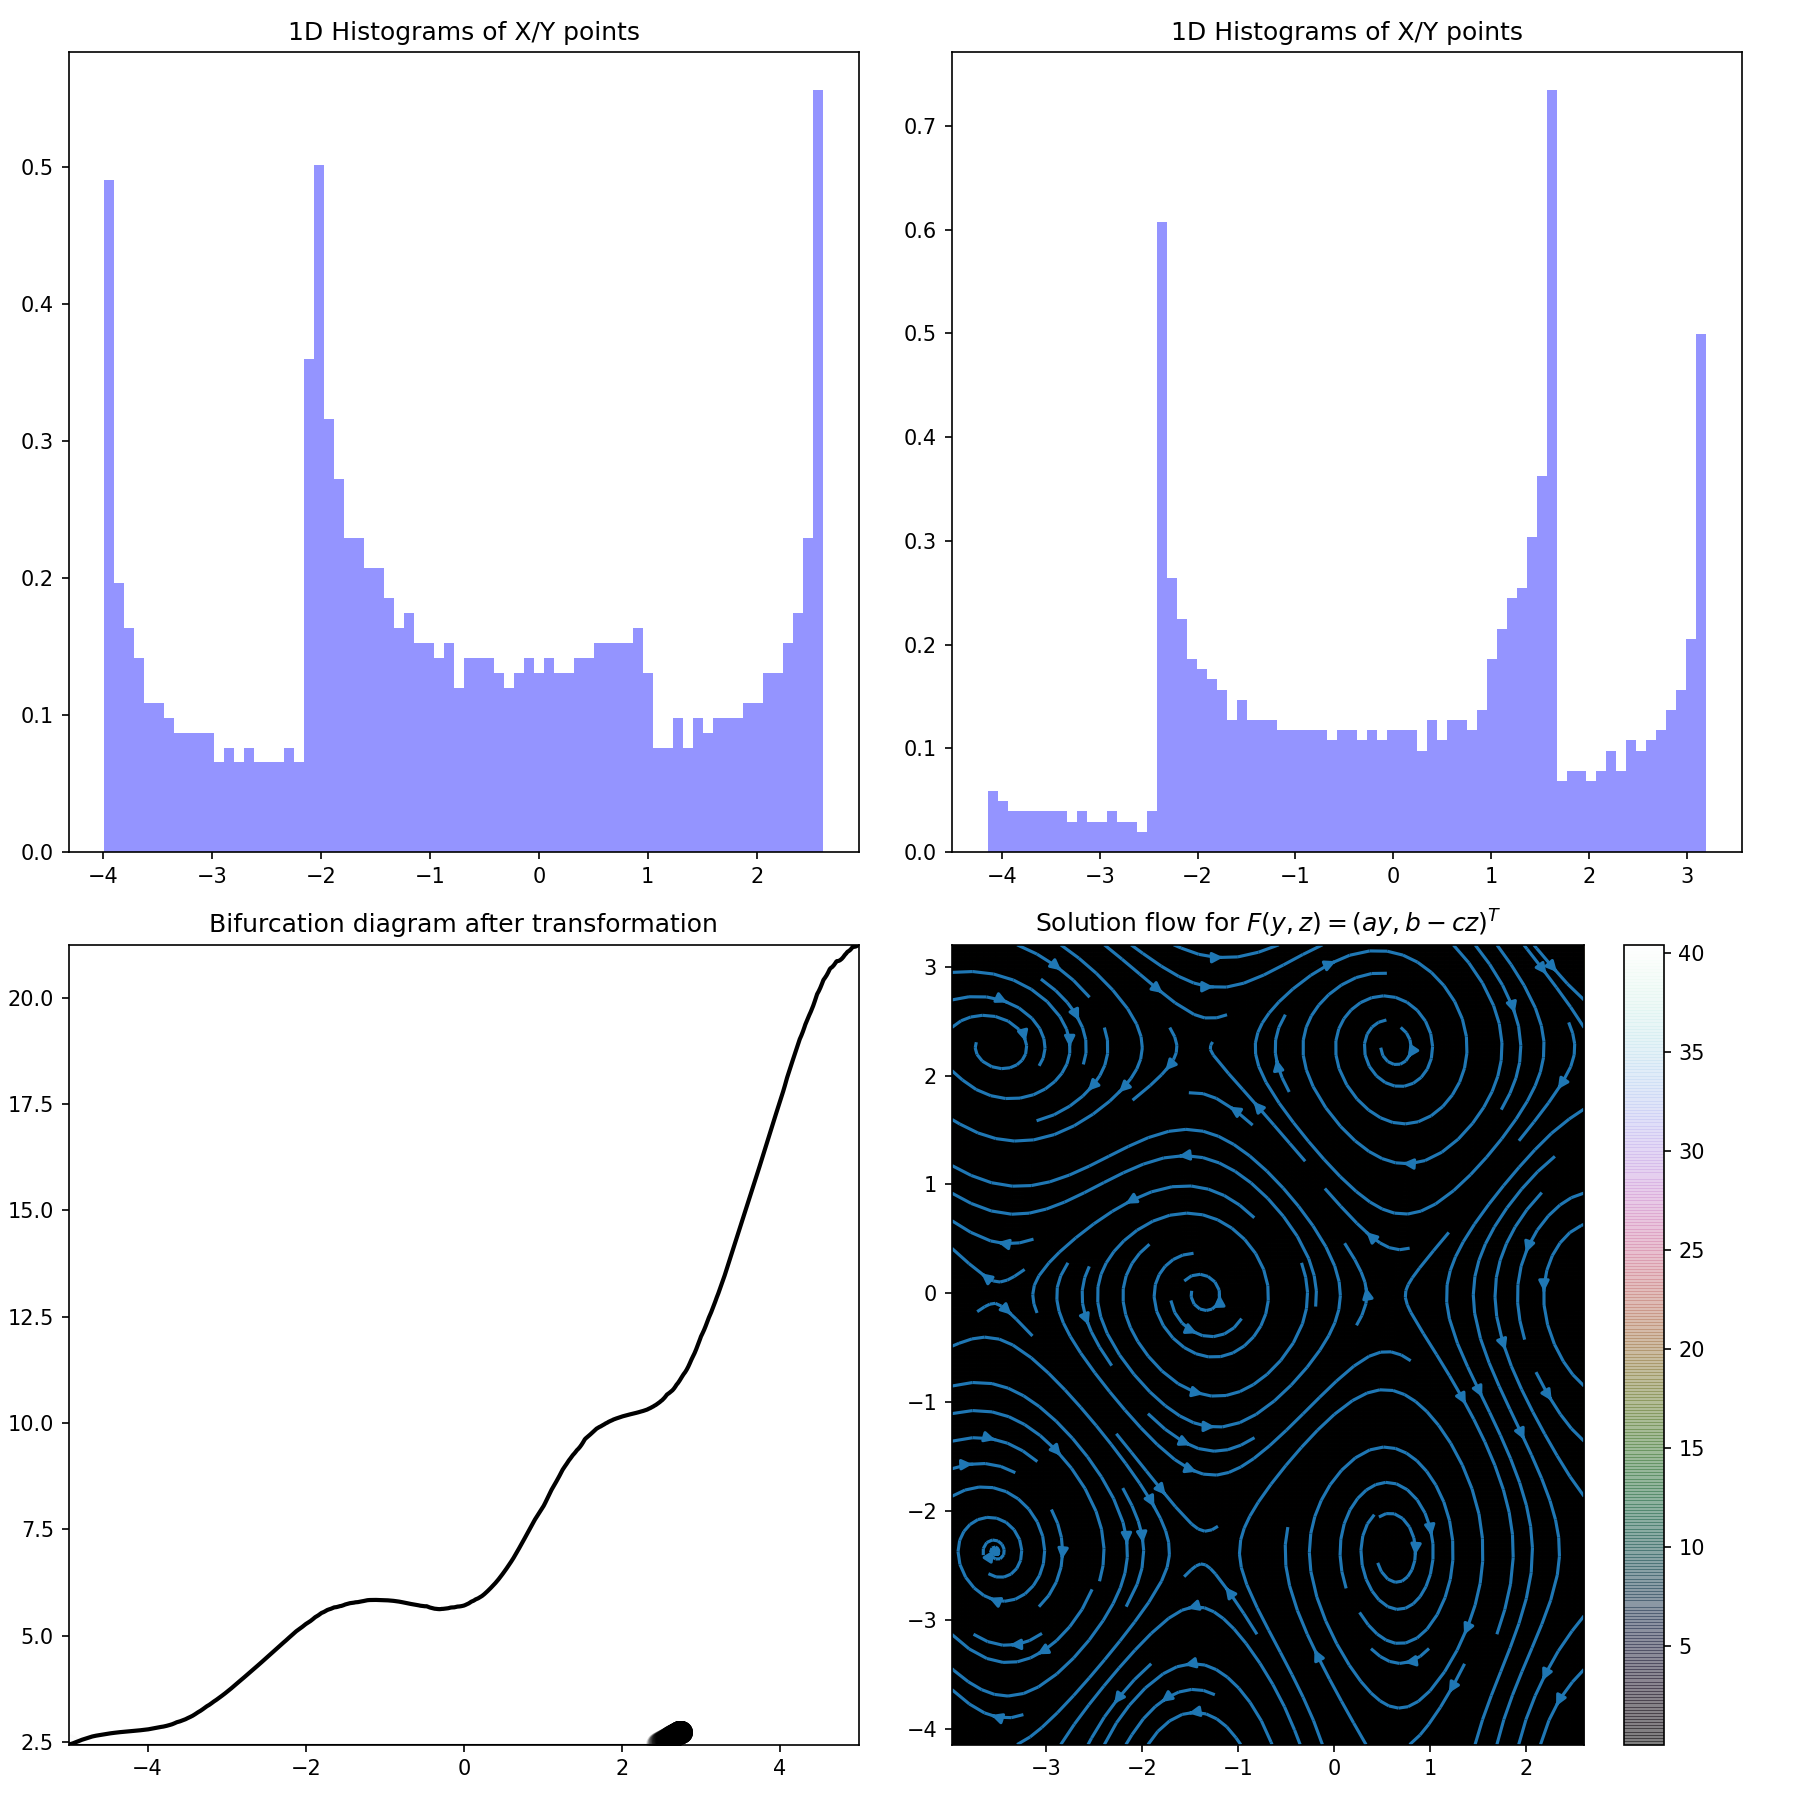
\includegraphics[height=0.75\textheight]{../Images/RosslerAttractorSummary-TypeXY-Plot1D-A0-200B0-200C5-700-2021-10-27-044726.png}
\end{center}

\end{frame}

\begin{frame}[fragile]
\frametitle{Exploring the classical parameter solution (3D plots)}

The solution projected into the $XY$-plane (by setting $Z=0$) with the ``classic'' 
parameters $(a, b, c) = (0.2, 0.2, 5.7)$. \\ 
\begin{center}
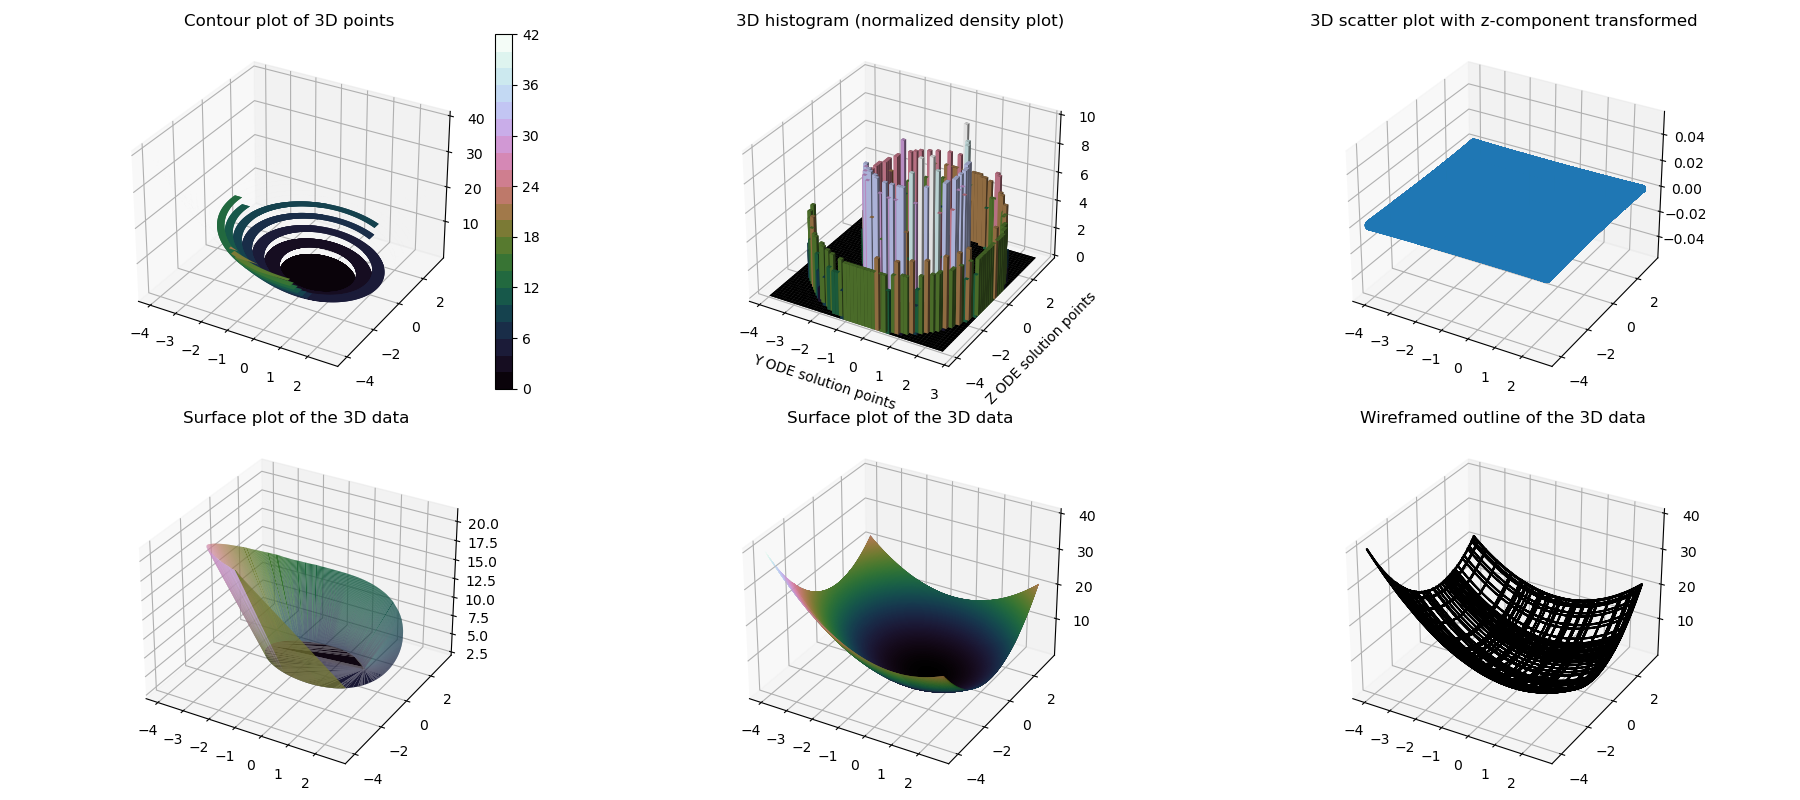
\includegraphics[width=0.95\textwidth]{../Images/RosslerAttractorSummary-TypeXY-Plot3D-A0-200B0-200C5-700-2021-10-27-044740.png}
\end{center}

\end{frame}

\begin{frame}[fragile]
\frametitle{Exploring the classical parameter solution (1D plots)}

The solution projected into the $YZ$-plane (by setting $X=0$) with the ``classic'' 
parameters $(a, b, c) = (0.2, 0.2, 5.7)$. \\ 
\begin{center}
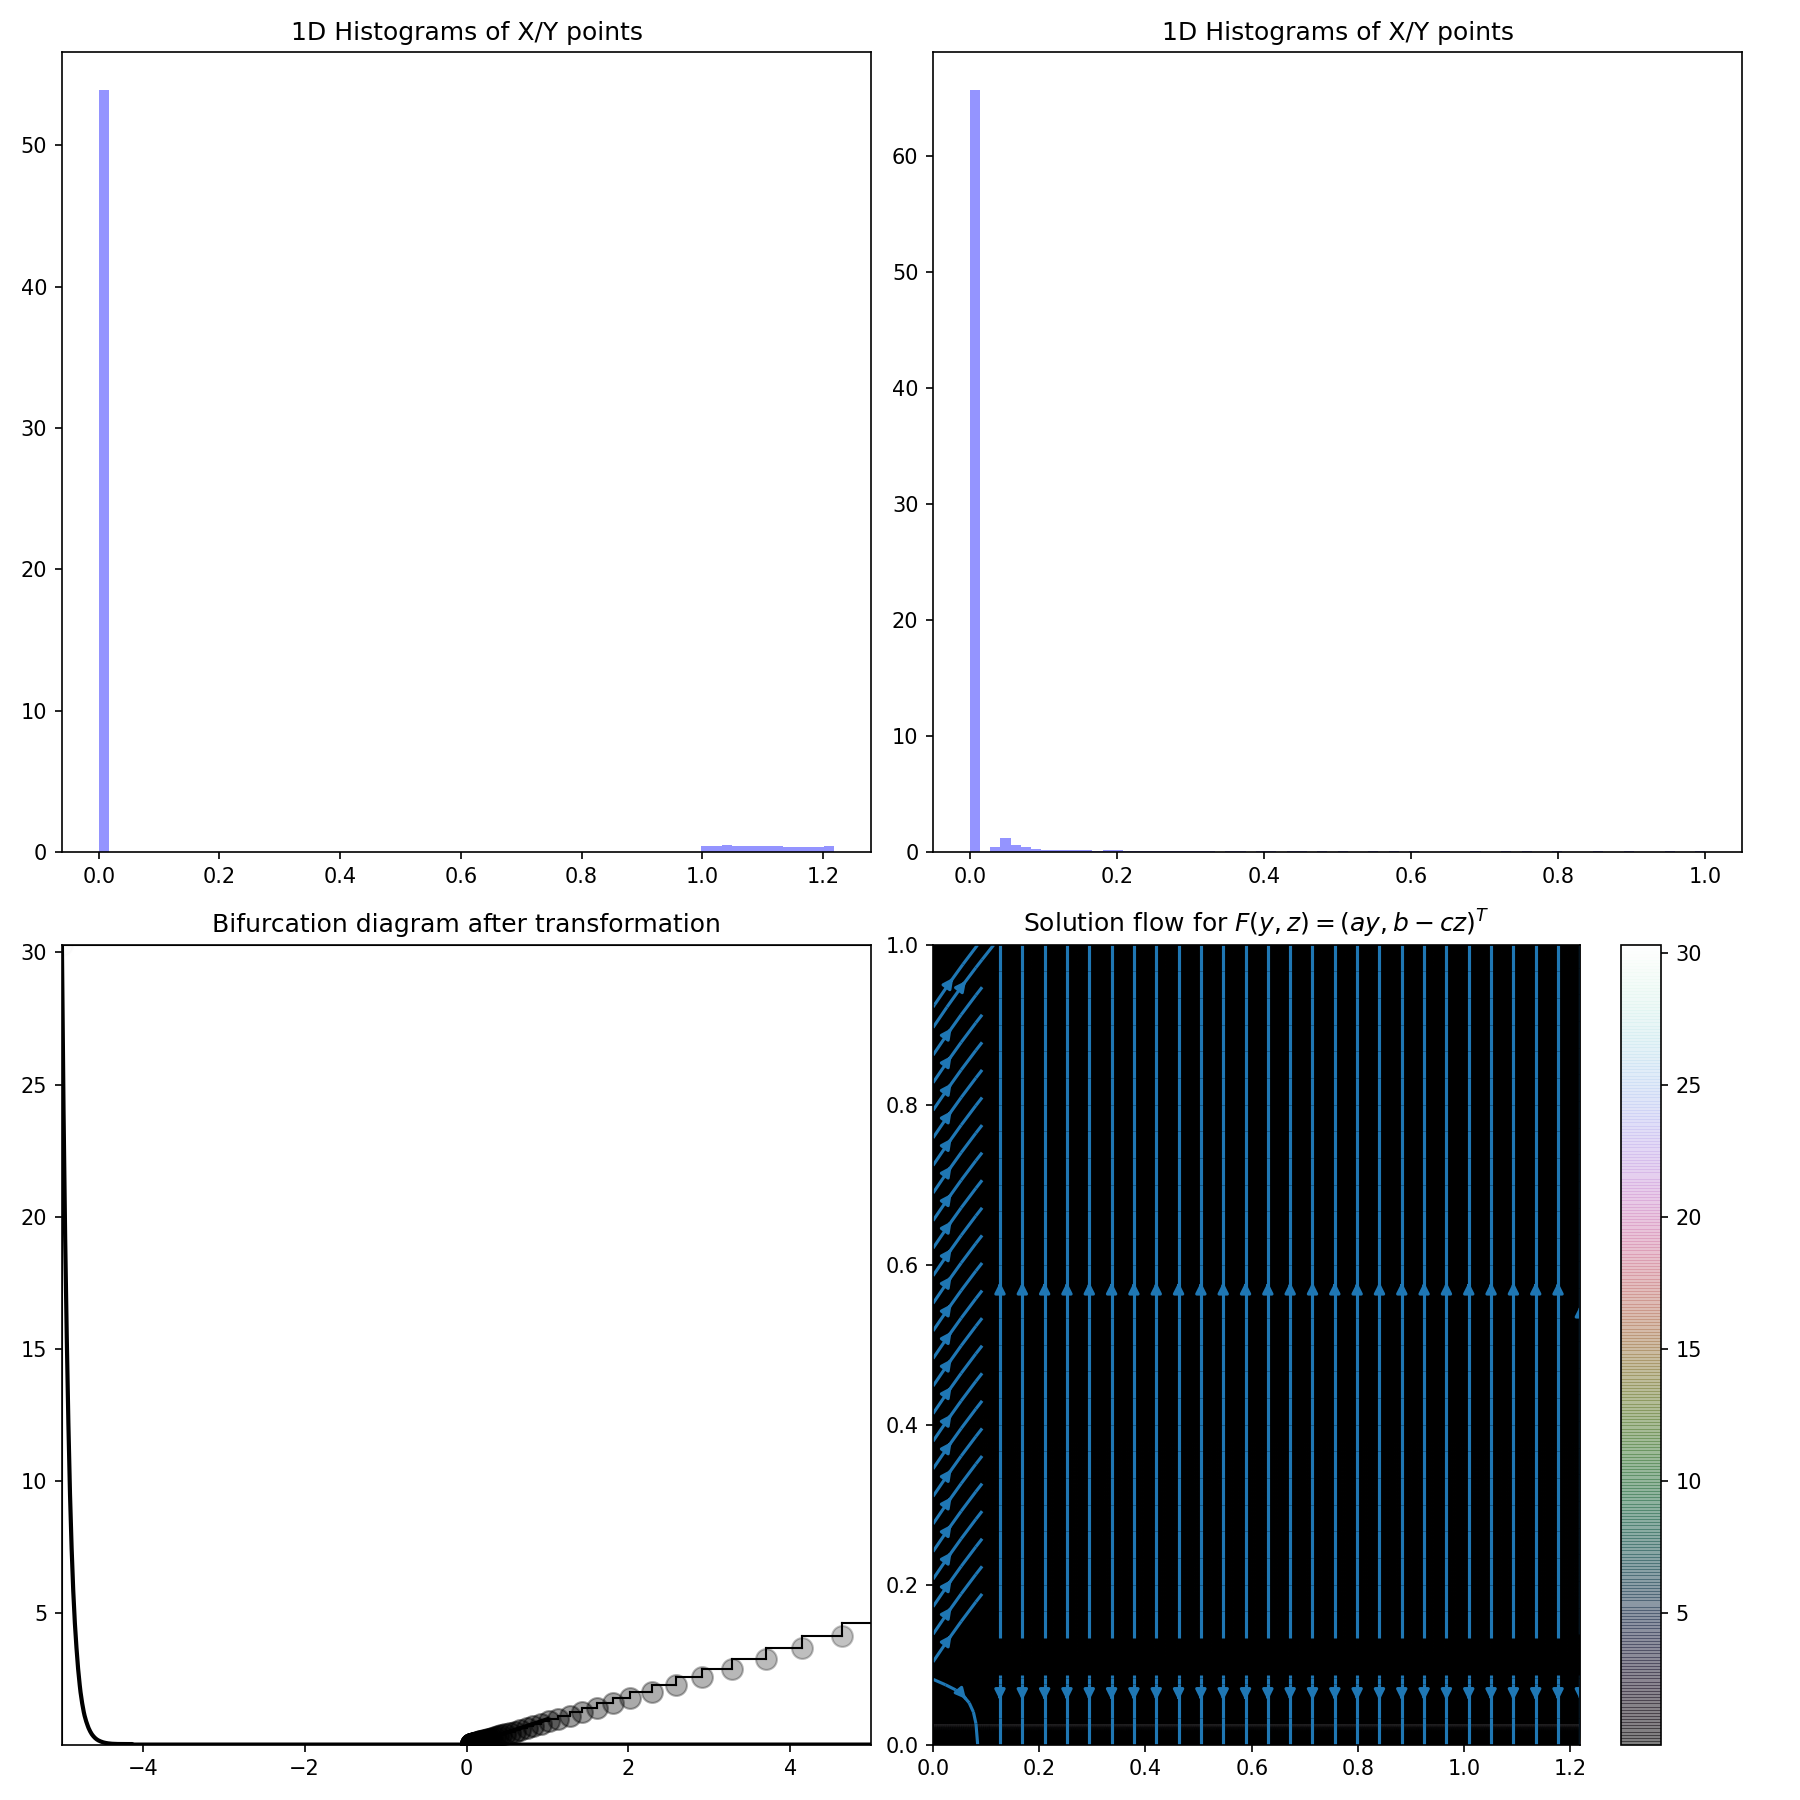
\includegraphics[height=0.75\textheight]{../Images/RosslerAttractorSummary-TypeYZ-Plot1D-A0-200B0-200C5-700-2021-10-27-045009.png}
\end{center}

\end{frame}

\begin{frame}[fragile]
\frametitle{Exploring the classical parameter solution (3D plots)}

The solution projected into the $YZ$-plane (by setting $X=0$) with the ``classic'' 
parameters $(a, b, c) = (0.2, 0.2, 5.7)$. \\ 
\begin{center}
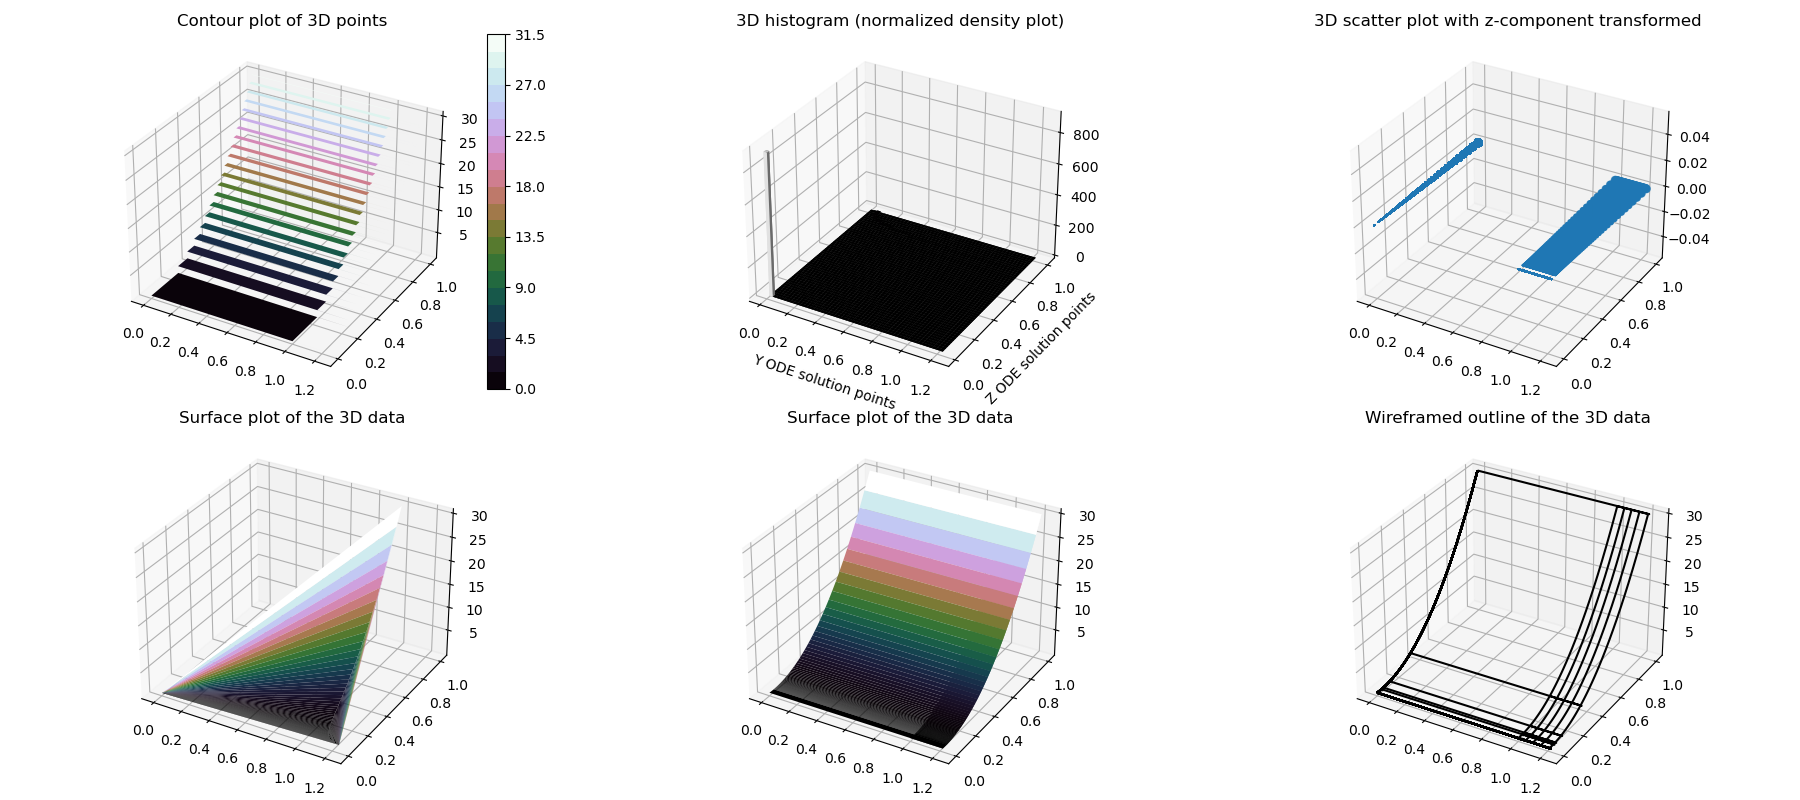
\includegraphics[width=0.95\textwidth]{../Images/RosslerAttractorSummary-TypeYZ-Plot3D-A0-200B0-200C5-700-2021-10-27-045026.png}
\end{center}

\end{frame}

\subsection{Modified experiment V1}

\begin{frame}
\frametitle{A modified experiment definition (Experiment V1)}

\begin{itemize} 

\item More so than a theoretically motivated example, we present Python3 source code for a numerical experiment 
      that can be generalized and extended for use in other related applications 
\item Consider the following generalization of the 1D-parameter \emph{Lyapunov coefficient} that results when 
     $v_0 \in \mathbb{R}^2$ is a fixed constant vector and $R(x, y, z)$ is the 2D R\"ossler system formed by 
     omitting the projection component: \\ 
     \[
     \lambda(a, b, c) := \frac{1}{N} \times \sum_{0 \leq i, j, k < N} \log\left\lvert \frac{\partial R}{\partial t}(x_i, y_j, z_k) \cdot v_0 \right\rvert. 
     \]
\item Since $\lambda(a, b, c)$ depends symbolically on the parameters $(a, b, c)$, we consider a relation on real values 
      of these parameters that restricts a grid of these parameters upon which we can form a plot. 
\item Then for the $(a, b, c) \in \mathbb{R}^3$ that satisfy this relation, we plot a \texttt{mathplotlib.pyplot.hexbin} 
      graph of $|\lambda(a, b, c)|$ on the Cartesian $y$-axis against the values of another function $\mathcal{T}_x(a, b, c)$ on the 
      $x$-axis

\end{itemize} 

\end{frame}

\begin{frame}
\frametitle{A modified experiment definition (Experiment V1)}

\begin{itemize} 

\item Limitations and incompatibility: The implementation was tricky in Python3 for a few reasons: 
      \begin{itemize} 
      \item There is considerable incompatibility in the types of the objects returned by large / mature Python3 libraries like 
            \texttt{sympy}, \texttt{scipy}, \texttt{numpy} and even within \texttt{sage} (the \emph{SageMath} CAS environment) 
      \item There is really no good way to solve a 3D system of ODEs when the solutions involve symbolic parameters 
            like the unevaluated indeterminates $(a, b, c)$ 
      \item Numerically evaluating the entire ODE solution for each possibility of $(a, b, c)$ is an inefficient, time-consuming 
            approach
      \end{itemize}

\end{itemize} 

\end{frame}


\begin{frame}[fragile]
\frametitle{Modified experiment V1 -- Variant \#1 (results)}

\begin{center}
\begin{code}
(sage) cd Examples/RosslerAttractor
(sage) run "RosslerGenLyapunovExponentExperiments.py"
\end{code}
\textbf{Variant 1:} 
In the projected $XY$-plane with linear (left) and logarithmic (right) scaling on the $X$-axis defined by 
$\mathcal{T}_x(a, b, c) := \frac{c}{a} + \frac{a^2}{c}$, subject to the restriction that 
$a^2+b^2+c^2 = 4$ (for real parameter values). \\ 
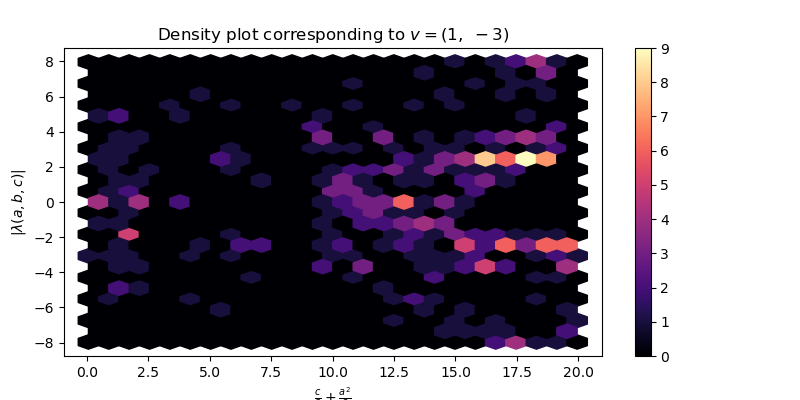
\includegraphics[width=0.49\textwidth]{../Images/RosslerAttractorExpt1-Variant1-linearscale-TypeXY-2021-10-27-025740.png}
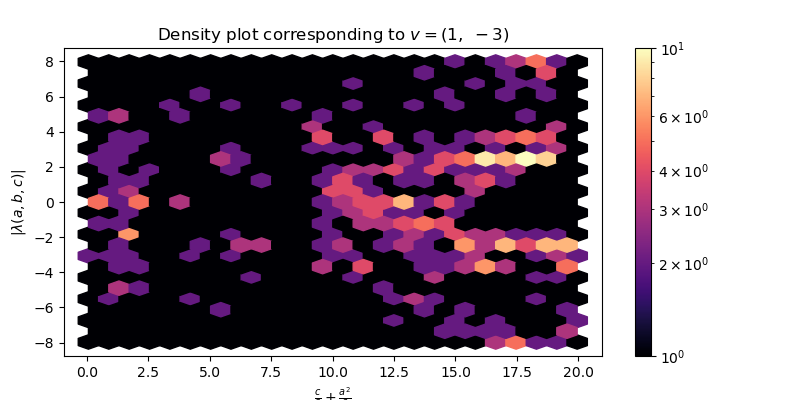
\includegraphics[width=0.49\textwidth]{../Images/RosslerAttractorExpt1-Variant1-logscale-TypeXY-2021-10-27-025253.png}
\end{center}

\end{frame}

\begin{frame}[fragile]
\frametitle{Modified experiment V1 -- Variant \#2 (results)}

\begin{center}
\begin{code}
(sage) cd Examples/RosslerAttractor
(sage) run "RosslerGenLyapunovExponentExperiments.py"
\end{code}
\textbf{Variant 2:} 
In the projected $XY$-plane with linear (left) and logarithmic (right) scaling on the $X$-axis defined by 
$\mathcal{T}_x(a, b, c) := \frac{c}{a} + \frac{a^2}{c}$, subject to the restriction that 
$(a-0.2)^4-(b^2-0.2)^3+2 (c-5.7)^2 = 4$ (for real parameter values). \\ 
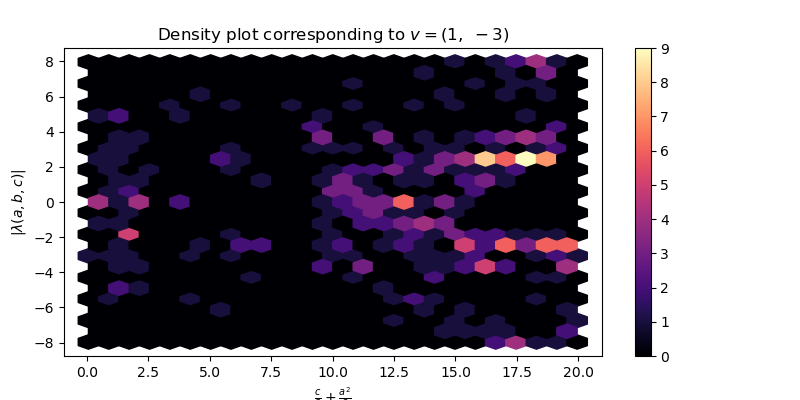
\includegraphics[width=0.49\textwidth]{../Images/RosslerAttractorExpt1-Variant2-linearscale-TypeXY-2021-10-27-025531.png}
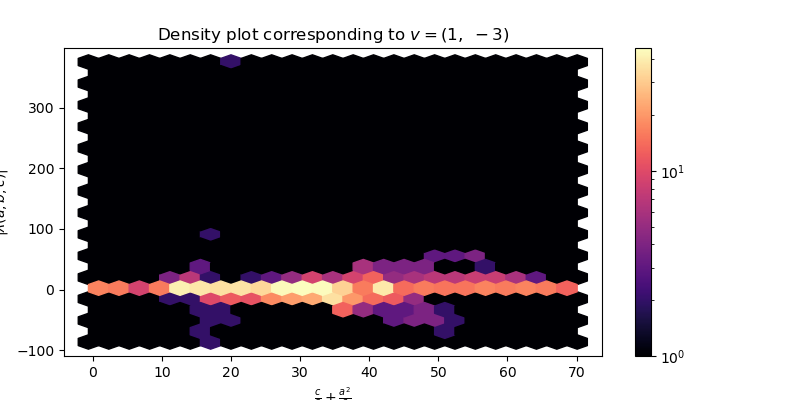
\includegraphics[width=0.49\textwidth]{../Images/RosslerAttractorExpt1-Variant2-logscale-TypeXY-2021-10-27-025057.png}
\end{center}

\end{frame}

\begin{frame}[fragile]
\frametitle{Modified experiment V1 -- Variant \#3 (results)}

\begin{center}
\begin{code}
(sage) cd Examples/RosslerAttractor
(sage) run "RosslerGenLyapunovExponentExperiments.py"
\end{code}
\textbf{Variant 3:} 
In the projected $XY$-plane with linear (right) and logarithmic (left) scaling on the $X$-axis defined by 
$\mathcal{T}_x(a, b, c) := a + b + c$, subject to the restriction that 
$(a+b+c)^2 = 3$ (for real parameter values). \\ 
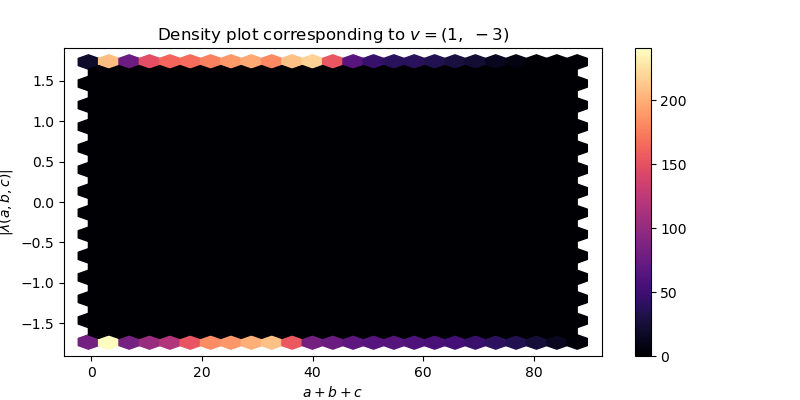
\includegraphics[width=0.49\textwidth]{../Images/RosslerAttractorExpt1-Variant3-linearscale-TypeXY-2021-10-27-042004.png}
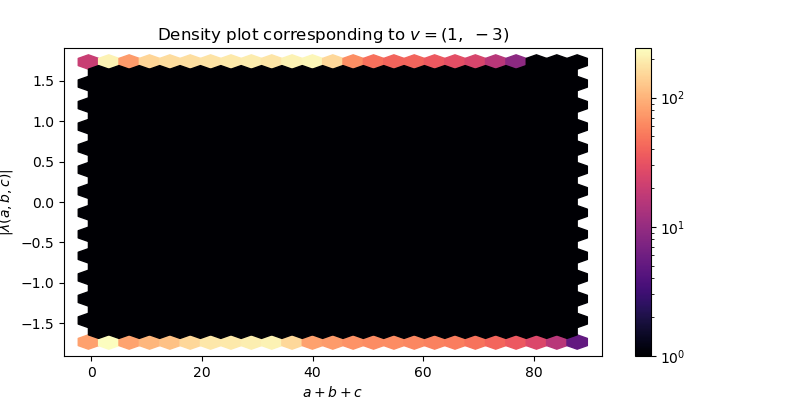
\includegraphics[width=0.49\textwidth]{../Images/RosslerAttractorExpt1-Variant3-logscale-TypeXY-2021-10-27-033310.png}
\end{center}

\end{frame}

\begin{frame}[fragile]
\frametitle{Modified experiment V1 -- Variant \#4 (results)}

\begin{center}
\begin{code}
(sage) cd Examples/RosslerAttractor
(sage) run "RosslerGenLyapunovExponentExperiments.py"
\end{code}
\textbf{Variant 4:} 
In the projected $XY$-plane with linear (right) and logarithmic (left) scaling on the $X$-axis defined by 
$\mathcal{T}_x(a, b, c) := abc$, subject to the restriction that 
$(a+b+c)^2 = 3$ (for real parameter values). \\ 
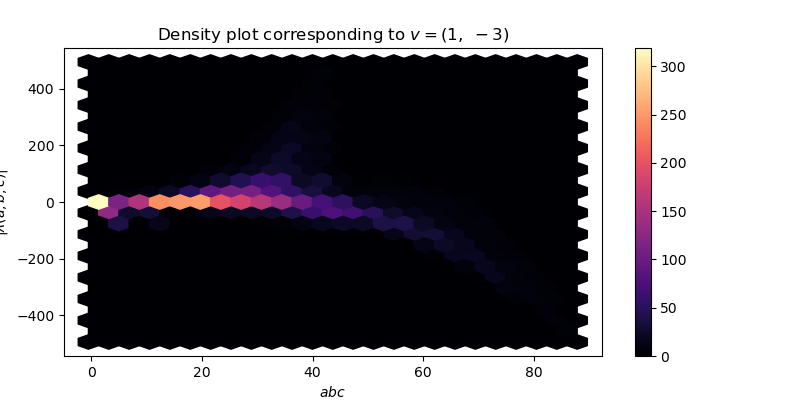
\includegraphics[width=0.49\textwidth]{../Images/RosslerAttractorExpt1-Variant4-linearscale-TypeXY-2021-10-27-040705.png}
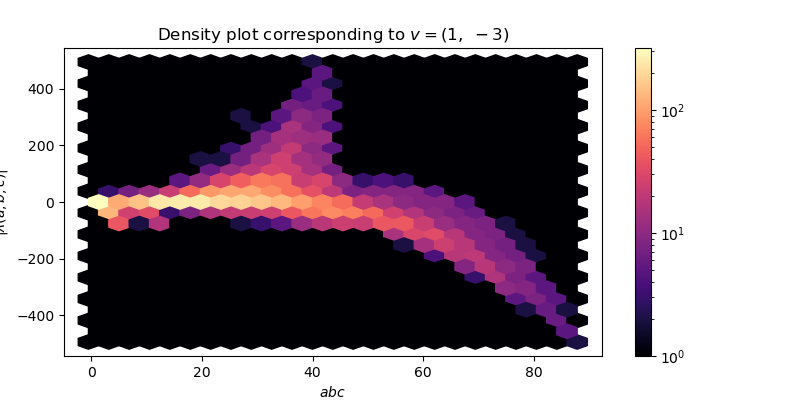
\includegraphics[width=0.49\textwidth]{../Images/RosslerAttractorExpt1-Variant4-logscale-TypeXY-2021-10-27-035400.png}
\end{center}

\end{frame}

\begin{frame}[fragile]
\frametitle{Modified experiment V1 -- Variant \#5 (results)}

\begin{center}
\begin{code}
(sage) cd Examples/RosslerAttractor
(sage) run "RosslerGenLyapunovExponentExperiments.py"
\end{code}
\textbf{Variant 5 (Parameterizations of a heart shape in the plane):} 
In the projected $XY$-plane with linear (right) and logarithmic (left) scaling on the $X$-axis defined by 
$\mathcal{T}_x(a, b, c) :=13\cos(T)-5\cos(2T)-2\cos(3T)-\cos(4T)$ with $T \equiv a + b + c$, 
subject to the restriction that $(a^2+b^2+ac)^2 = c^2(a^2+b^2)$. \\ 
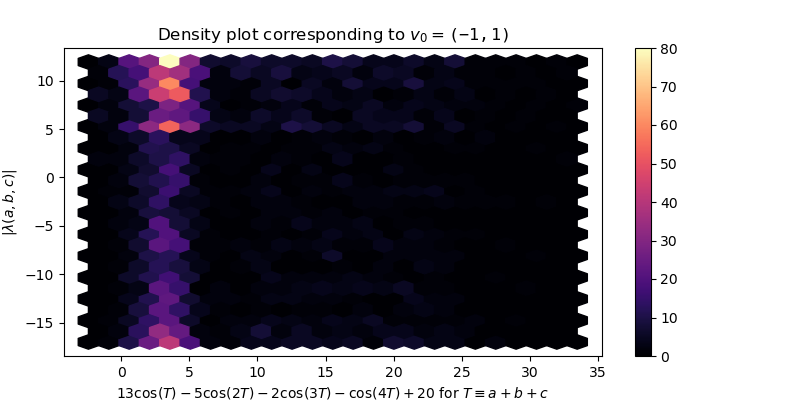
\includegraphics[width=0.49\textwidth]{../Images/RosslerAttractorExpt1-Variant265242-linearscale-TypeXY-2021-10-27-095559.png}
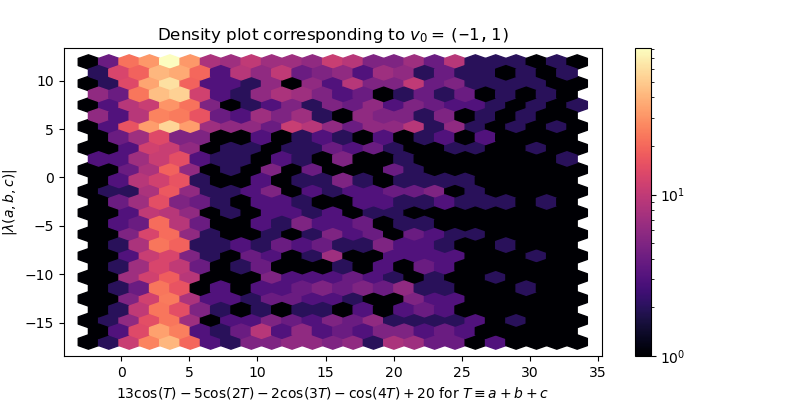
\includegraphics[width=0.49\textwidth]{../Images/RosslerAttractorExpt1-Variant265242-logscale-TypeXY-2021-10-27-095541.png}
\end{center}

\end{frame}

\subsection{Modified experiment V1}

\begin{frame}
\frametitle{Experiment V2: Problem setup}

\begin{itemize} 

\item The hexagon density plots that resulted in seemingly random choices of the $X$-axis functions 
      and relations between the parameters suggest that there is more hidden underneath 
      (e.g., some semblance of regularity to be quantified in) the definition of 
      $\lambda(a, b, c)$ 
\item For this experiment, we consider the projected system to $XY$ components (setting $Z=0$) 
\item The resulting 2D ODE system only depends on one parameter: $a$ 
\item So we consider the following function: 
      \[
      \lambda(a, u) := \frac{1}{N^2} \times \sum_{0 \leq i, j, k < N} \log\left\lvert 
      (-y_{N,j}, x_{N,i}+ay_{N,j}) \cdot (u, -1)\right\rvert. 
      \]
\item Note that we consider a uniform grid for $t$ such that the difference between the 
      $N$ distinct time points goes to zero as $N \rightarrow \infty$. Then 
      $(x_{N,i}, y_{N,j}) = (x(t_{N,i}), y(t_{N,j}))$ where the LHS functions are also implicitly functions 
      of the (indeterminate) parameter: $a$
\end{itemize}

\end{frame}

\begin{frame}
\frametitle{Experiment V2: Problem setup (cont'd)}

\begin{itemize} 

\item Some arithmetic yields that 
      \begin{align*}
      \lambda(a, u) & = \frac{1}{N} \times 
           \underset{ := \lambda_{0,N}(a)}{\underbrace{\log\left[\prod_{0 \leq i < N} |x_{N,i}|\right]}} + 
           \frac{1}{N^2} \times \log\left[\prod_{0 \leq i,j < N} \left\lvert 1 + 
           \frac{(u+a)y_{N,j}}{x_{N,i}}\right\rvert\right]. 
      \end{align*}
\item Want to verify numerically that the following limit exists for each $a, u \in (-\infty, \infty)$:  
      \[
      \lambda_0(a) = \lim_{N \rightarrow \infty} \frac{\lambda_{0,N}(a)}{N}. 
      \]
\item We also pose an ansatz that (for at least some $a,u$) we should get a limiting probability 
      measure when any $(i, j) \in [0, N)^2 \bigcap \mathbb{Z}^2$ is selected uniformly at random 
      \[
      \nu(a, u; t) = \lim_{N \rightarrow \infty} \mathbb{P}\left[\frac{y_{N,j}}{x_{N,i}} = t\right], t \in \mathbb{R}
      \]

\end{itemize} 

\end{frame}

\begin{frame}
\frametitle{Experiment V2: Problem setup (cont'd)}

\begin{itemize} 

\item When this happens, we have that 
      \begin{align*}
      \lambda(a, u) & = \lambda_0(a) + \int_{-\infty}^{\infty} \log\left\lvert 1 + (u+a)t \right\rvert 
           \nu(a, u; t) dt \\ 
           & = \lambda_0(a) + \int_{\tau_{\ell}(a, u)}^{\tau_u(a, u)} \log\left\lvert 1 + (u+a)t \right\rvert 
           \nu(a, u; t) dt \\ 
           & = \lambda_0(a) + 
           \log\left\lvert 1 + (u+a)t \right\rvert \left(\mathbb{P}\left[\Theta \leq t\right] - 1\right)
           \Biggr\rvert_{\tau_{\ell}(a, u)}^{\tau_u(a, u)} \\ 
           & \phantom{=\ } + 
           \int_{\tau_{\ell}(a, u)}^{\tau_u(a, u)} \frac{(u+a) \mathbb{P}\left[\Theta \geq t\right]}{1+(u+a)t} dt, 
      \end{align*} 
      where we have $-\infty < \tau_{\ell}(a, u), \tau_u(a, u) < \infty$ (the measure has finite support; 
      justified by examining other special cases of this system) and $\Theta$ is a random variable 
      distributed such that $\nu(a, u; t)$ is its PDF 

\end{itemize}

\end{frame}

\begin{frame}[fragile]
\frametitle{Experiment V2: Numerical methods towards the ansatz}

\begin{center}
\begin{code}
(sage) cd Examples/RosslerAttractor
(sage) run "RosslerGenLyapunovExponentExperiments2.py"
\end{code}
\textbf{Note:} It is \emph{very} time consuming to run the above script for a fine-grained mesh 
that gives the $N \rightarrow \infty$ behavior. These plots show the numerical results with the 
plot grid taken on a mesh with of granularity 
$(h, \Delta a) = (0.075, 0.075)$. \\ 
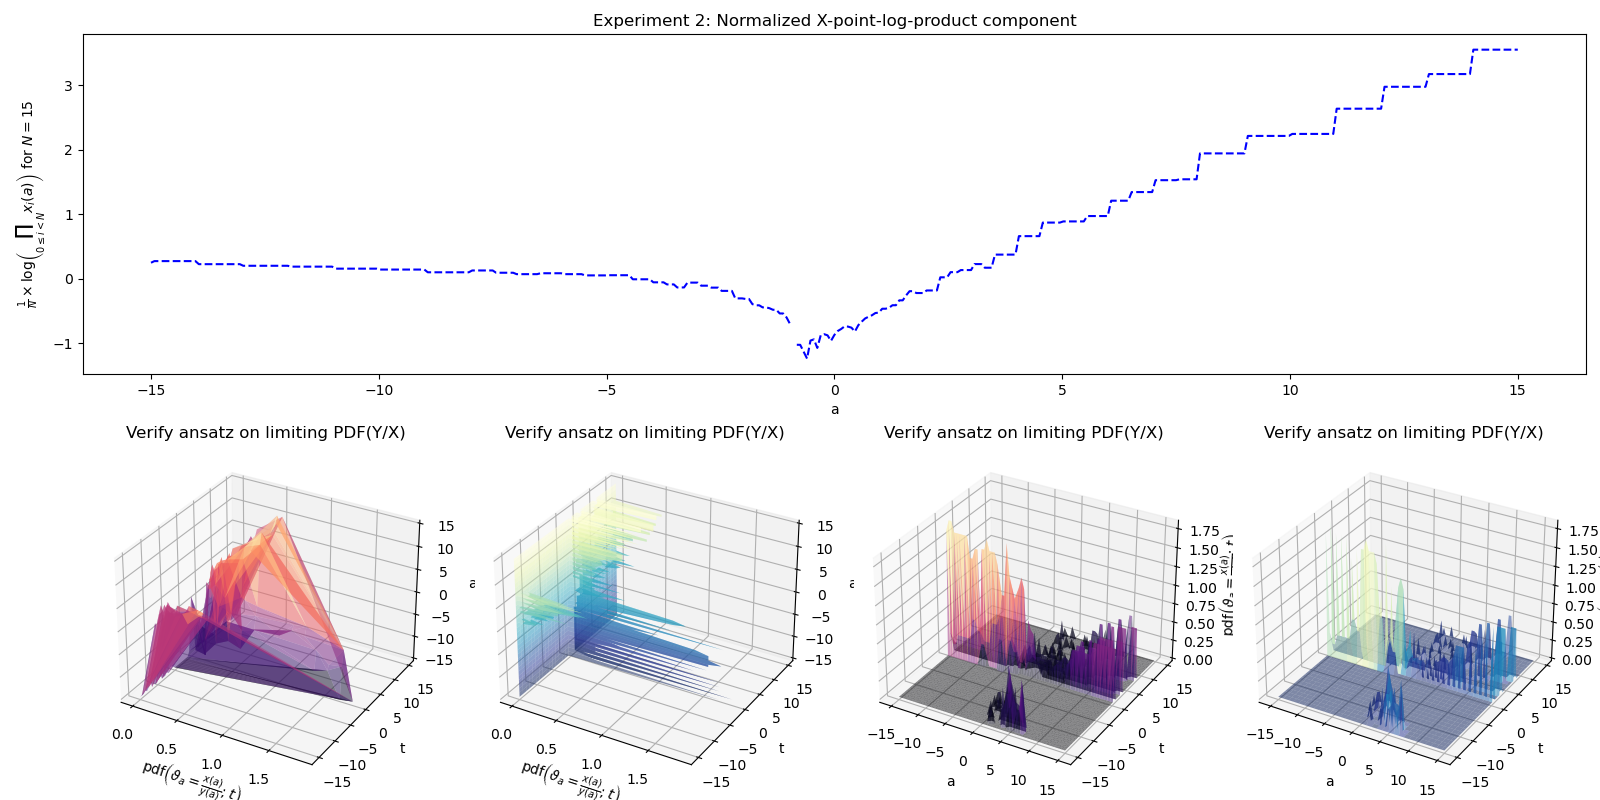
\includegraphics[height=0.65\textheight]{../Images/RosslerAttractorExpt2-2021-10-28-031737.png}
\end{center}

\end{frame}

\begin{frame}
\frametitle{Experiment V2: Observations and open questions}

\begin{itemize} 

\item If we witness the convergence of $\lambda_0(a)$ and $\nu(a, u; t)$ to a probability measure, 
      are there then subsets of such 
      measure inducing parameters where we get particularly ``nice'' distributions? 
\item As is typical with chaotic attractor systems, we should (probably?) expect that for any 
      fixed $(a, u)$ where we get this convergence, there should be some 
      ``sweet spot'' $\widehat{P} = (a_0, u_0)$ such that $(a, u)$ is in a small neighborhood of 
      $\widehat{P}$ and at the main point we find exquisite properties given the territory. 
\item In running the Python script used to generate the plots on the previous slide, 
      we have had to exclude singularies for several $a$ where the ratio 
      $\vartheta_{N,i,j} = y_{N,j}(a) / x_{N,i}(a) = +\infty$ blows up. What does this indicate? 

\end{itemize}

\end{frame}

\section{Concluding Remarks} 

\begin{frame}
\frametitle{Concluding remarks and discussion} 

     \Huge{\centerline{The End}}\smallskip
     \Large{\centerline{Questions?}}\smallskip
     \Large{\centerline{Comments?}}\smallskip
     \Large{\centerline{Feedback?}}\bigskip
     \Huge{\centerline{Thank you for attending!}} 

\end{frame}

\begin{frame}[t,allowframebreaks] 
\frametitle{References} 

\footnotesize 
\begin{thebibliography}{10}

\bibitem{CHAOS-BOOK} 
K.~T.~Alligood, T.~D.~Sauer and J.~A.~Yorke. 
\emph{CHAOS: An introduction to dynamical systems} 
(cf.\ Chapter 6: \emph{Chaotic attractors}). 
Springer Textbooks in Mathematical Sciences, New York, 1997. 

\bibitem{WIKI-EULER-METHOD}
\emph{Euler method}. \url{https://en.wikipedia.org/wiki/Euler_method}

\bibitem{WIKI-LINEAR-MULTISTEP-METHOD} 
\emph{Linear multistep method}. \url{https://en.wikipedia.org/wiki/Linear_multistep_method} 

\bibitem{CATTR-SURVEY} 
C.~Robinson. \emph{What is a chaotic attractor?} 
\url{https://sites.math.northwestern.edu/~clark/publications/chaos.pdf} (2021)

\bibitem{WIKI-ROSSLER-ATTR}
\emph{R\"ossler attractor}. \url{https://en.wikipedia.org/wiki/R\"ossler_attractor}

\bibitem{WIKI-RK-METHOD} 
\emph{Runge-Kutta method}. \url{https://en.wikipedia.org/wiki/Runge-Kutta_methods} 

\end{thebibliography}

\end{frame} 

%----------------------------------------------------------------------------------------

\end{document} 

